\subsection{Results}

We did not have time to implement quantitative evaluation metrics beyond accuracy and loss, so we rely on our expertise to assess the quality of the generated tablatures.
Inference was conducted on the entire test set of 11,817 sequences.
The model achieved an accuracy of [VALUE TO FILL] on those sequences, with a corresponding loss of [VALUE TO FILL].
These values are very close to those observed on the validation set.

In this section, we showcase a selection of results from our experiments.
The examples were carefully chosen to demonstrate the model's ability to generate tablatures across different musical genres and diverse rhythmic guitar patterns.
We manually selected rhythmic guitar parts and extracted their corresponding tokens.
These examples originate from Songsterr \footnote{https://www.songsterr.com/} but are not part of the training dataset.
However, they belong to genres that are well-represented in DadaGP: various types of rock, metal and jazz funk.
Our work is the first to generate bass tablatures conditioned on rhythmic guitar parts, so we do not have other models to compare our results to.

\subsection{Examples}

% FIGURE EXAMPLE 1: METAL: ULTRA VOMIT RICARD PEINARD

\begin{figure}[!ht]
    \centering
    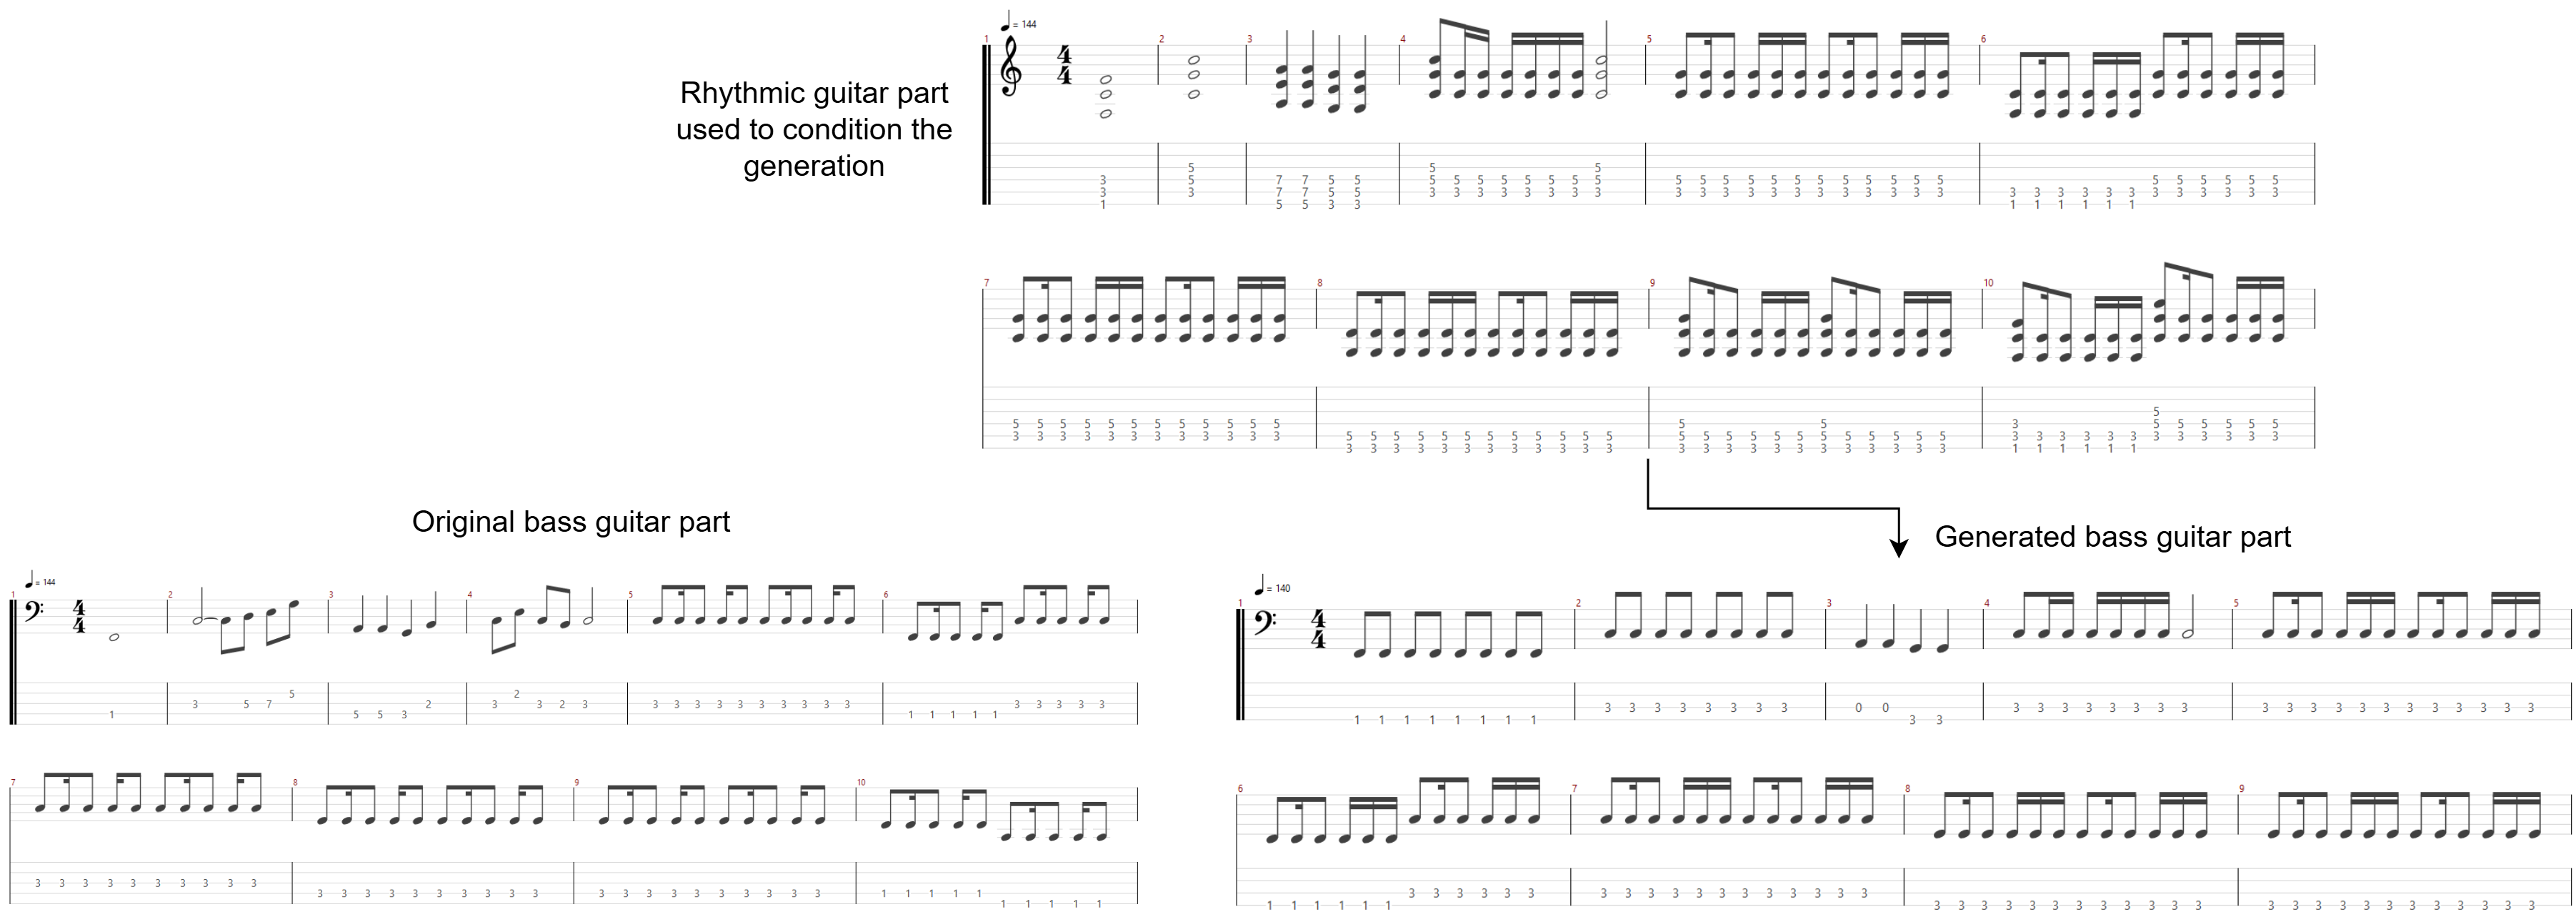
\includegraphics[width=\linewidth]{../images-figures/gen_ricard_peinard.png}
    \caption{Example of 9 measures generated by the model based on the rhythmic guitar part of the song "Ricard Peinard" by Ultra Vomit}
    \label{fig:gen_ricard_peinard}
\end{figure}

Figure \ref{fig:gen_ricard_peinard} shows an excerpt of bass tablatures generated by the model in the metal genre.
Bass guitar in metal music often plays a supportive role, doubling the rhythm guitar part at a lower pitch.
We also display the rhythmic guitar part and the original bass part.
Several criterion can be qualitatively used to evaluate the model's performance.
First, we can notice that the generated part is harmonically coherent with the rhythmic guitar part:
on the first measure the bass plays several F notes, while the rhythmic guitar plays a chord composed of F, C and G notes.
Rhythmically, the generated part either copies the rhythmic guitar or plays a simpler pattern such as a succession of eighth notes.
This is a correct outcome in the context of metal music, but needs to be further evaluated in other genres.
Finally, one may notice that the generated part is identical to the original bass part on measures 5 to 8.


% FIGURE EXAMPLE 2: INDIE ROCK: ARCTIC MONKEYS DO I WANNA KNOW

\begin{figure}[!ht]
    \centering
    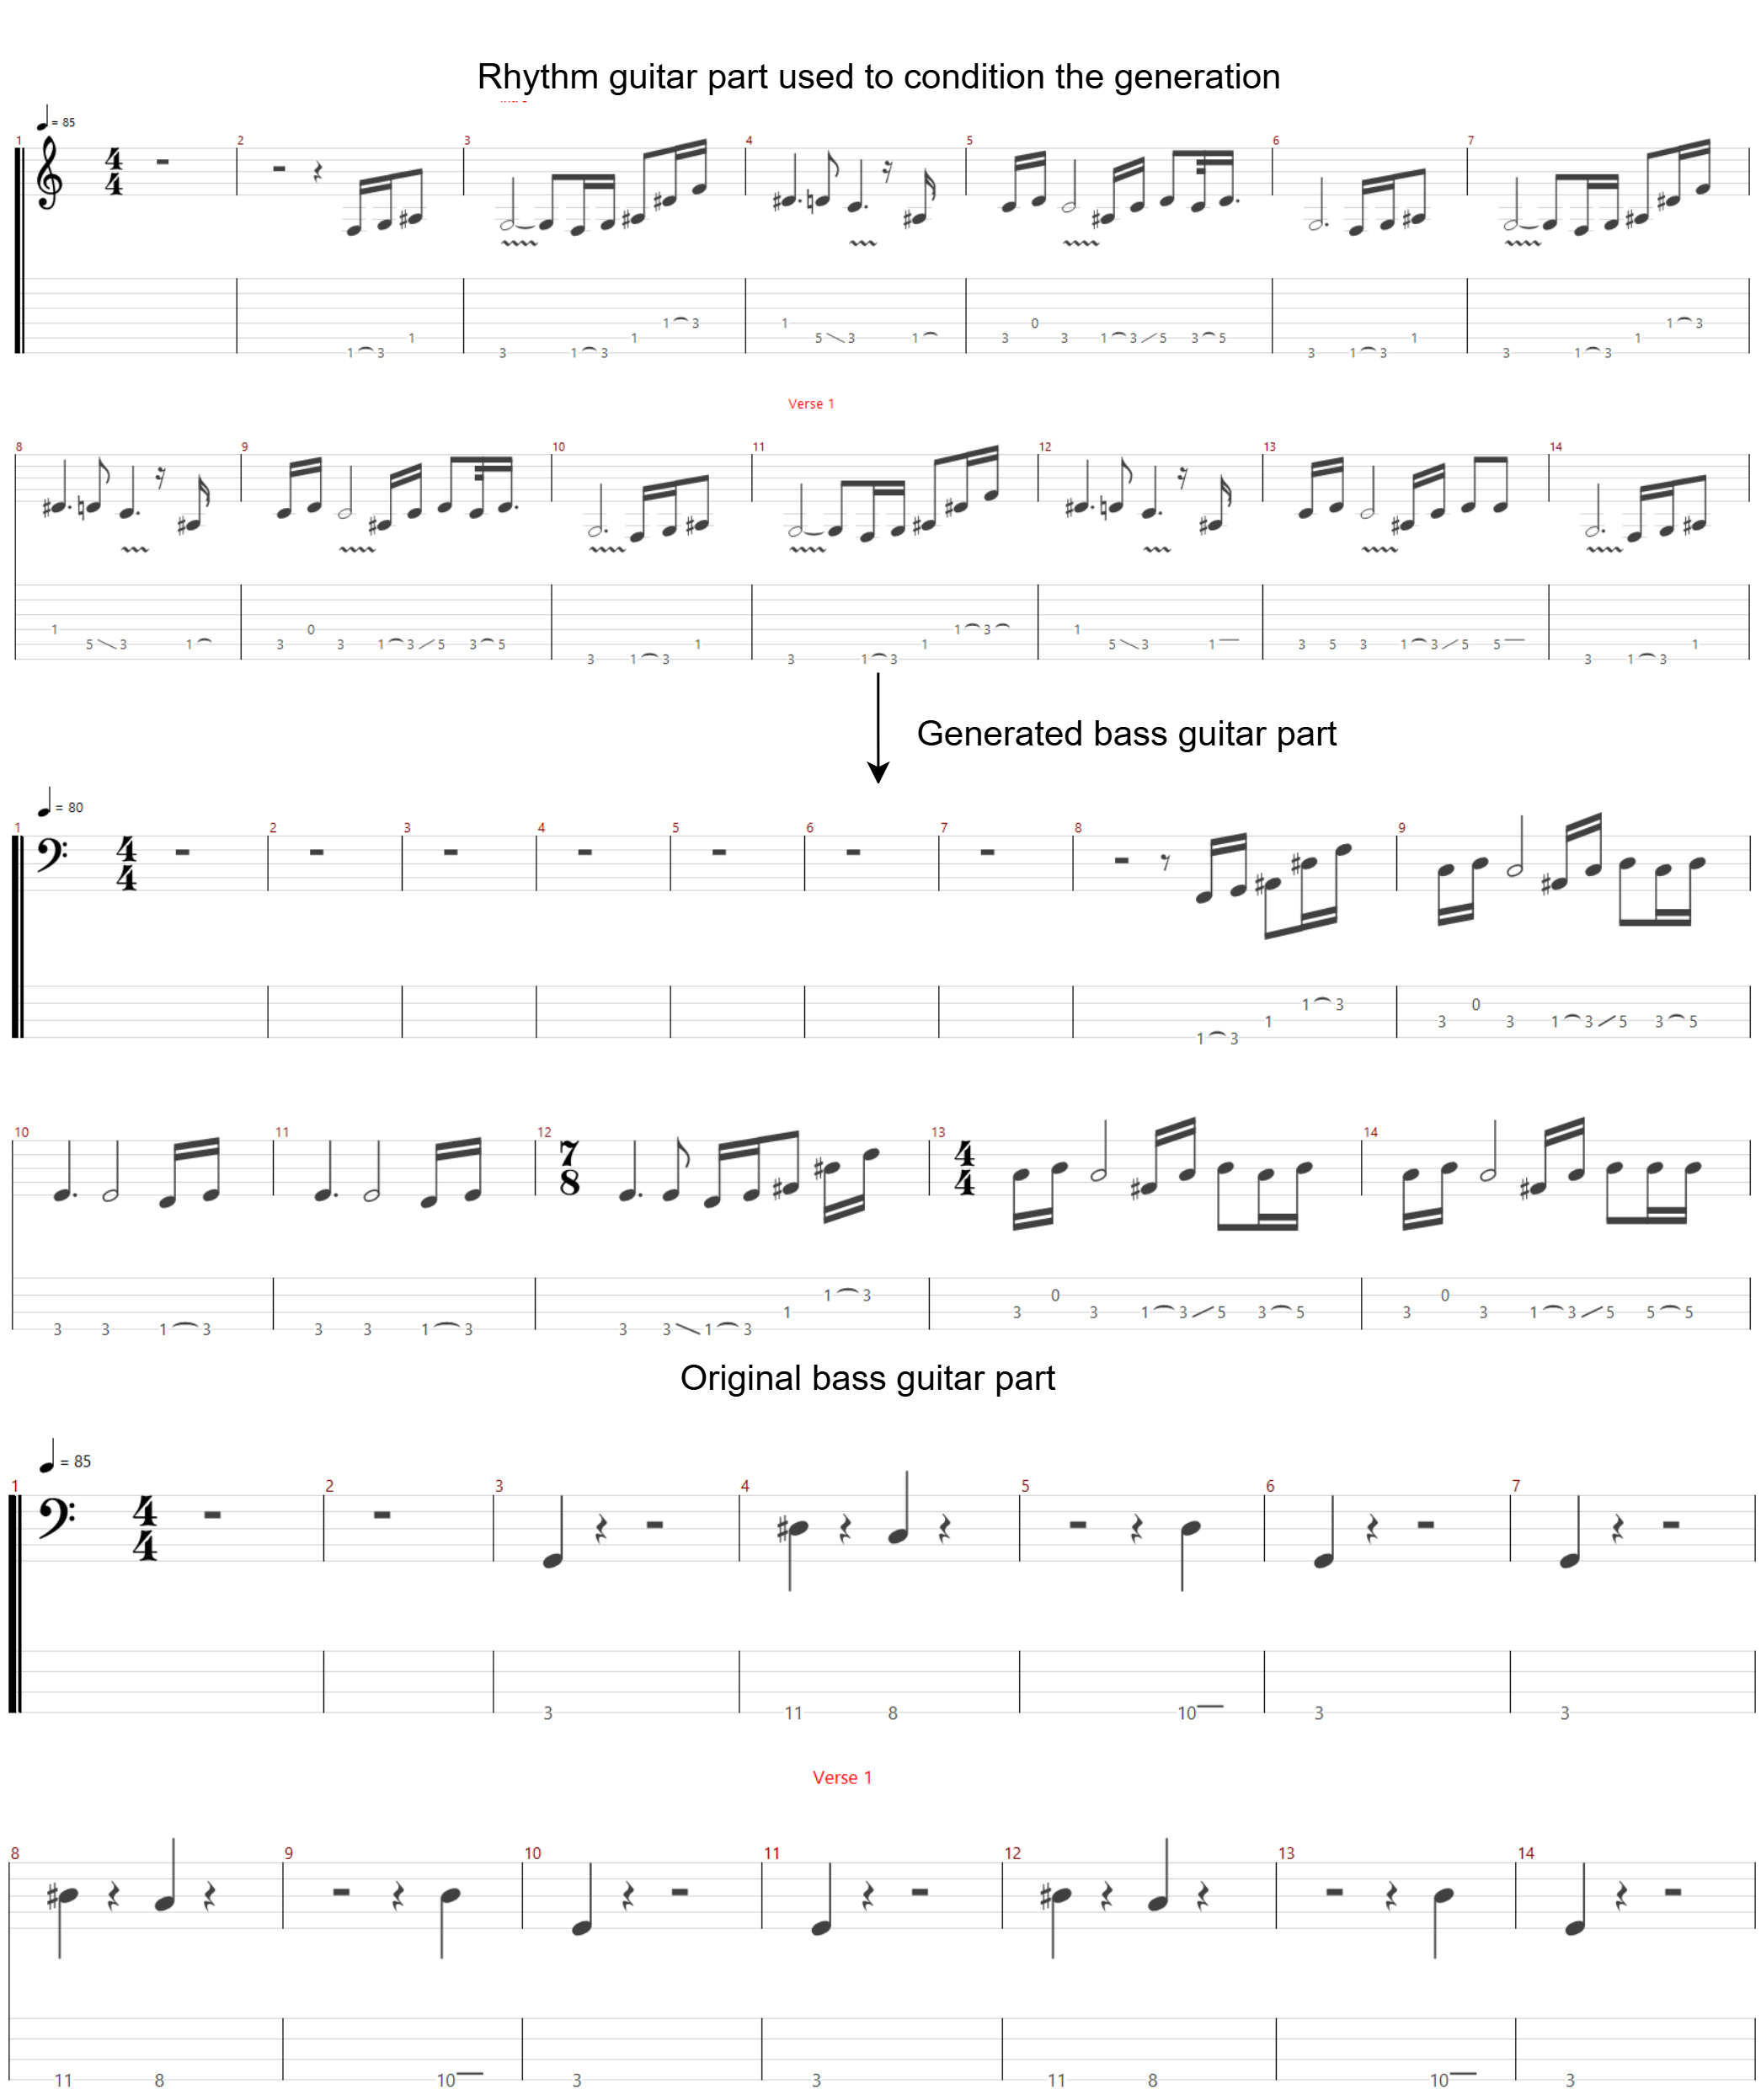
\includegraphics[width=\linewidth]{../images-figures/gen_arctic_monkeys.png}
    \caption{Example of 9 measures generated by the model based on the rhythmic guitar part of the song "Do I Wanna Know" by Arctic Monkeys}
    \label{fig:gen_arctic_monkeys}
\end{figure}

Figure \ref{fig:gen_arctic_monkeys} shows an excerpt of bass tablatures generated by the model in the indie rock genre.
Bass guitar's role in indie rock music is hard to define due to the genre's diversity.
However, this example remains particularly interesting as it demonstrates the model's tendency to copy the rhythmic guitar part even when very simple parts would be more appropriate.
Here the original bass part is basic yet essential, providing groove and structure to the song using quarter notes at specific onsets.
Nonetheless, the generated part remains harmonically and rhythmically coherent with the rhythmic guitar part.
This example also shows a recurrent issue in the model's inability to follow a time signature.
Here measure 12 becomes a 7/8 instead of a 4/4 (the model forgot an eighth note in the measure).


% FIGURE EXAMPLE 3: JAZZ FUNK: HERBIE HANCOCK SATURDAY NIGHT

\begin{figure}[!ht]
    \centering
    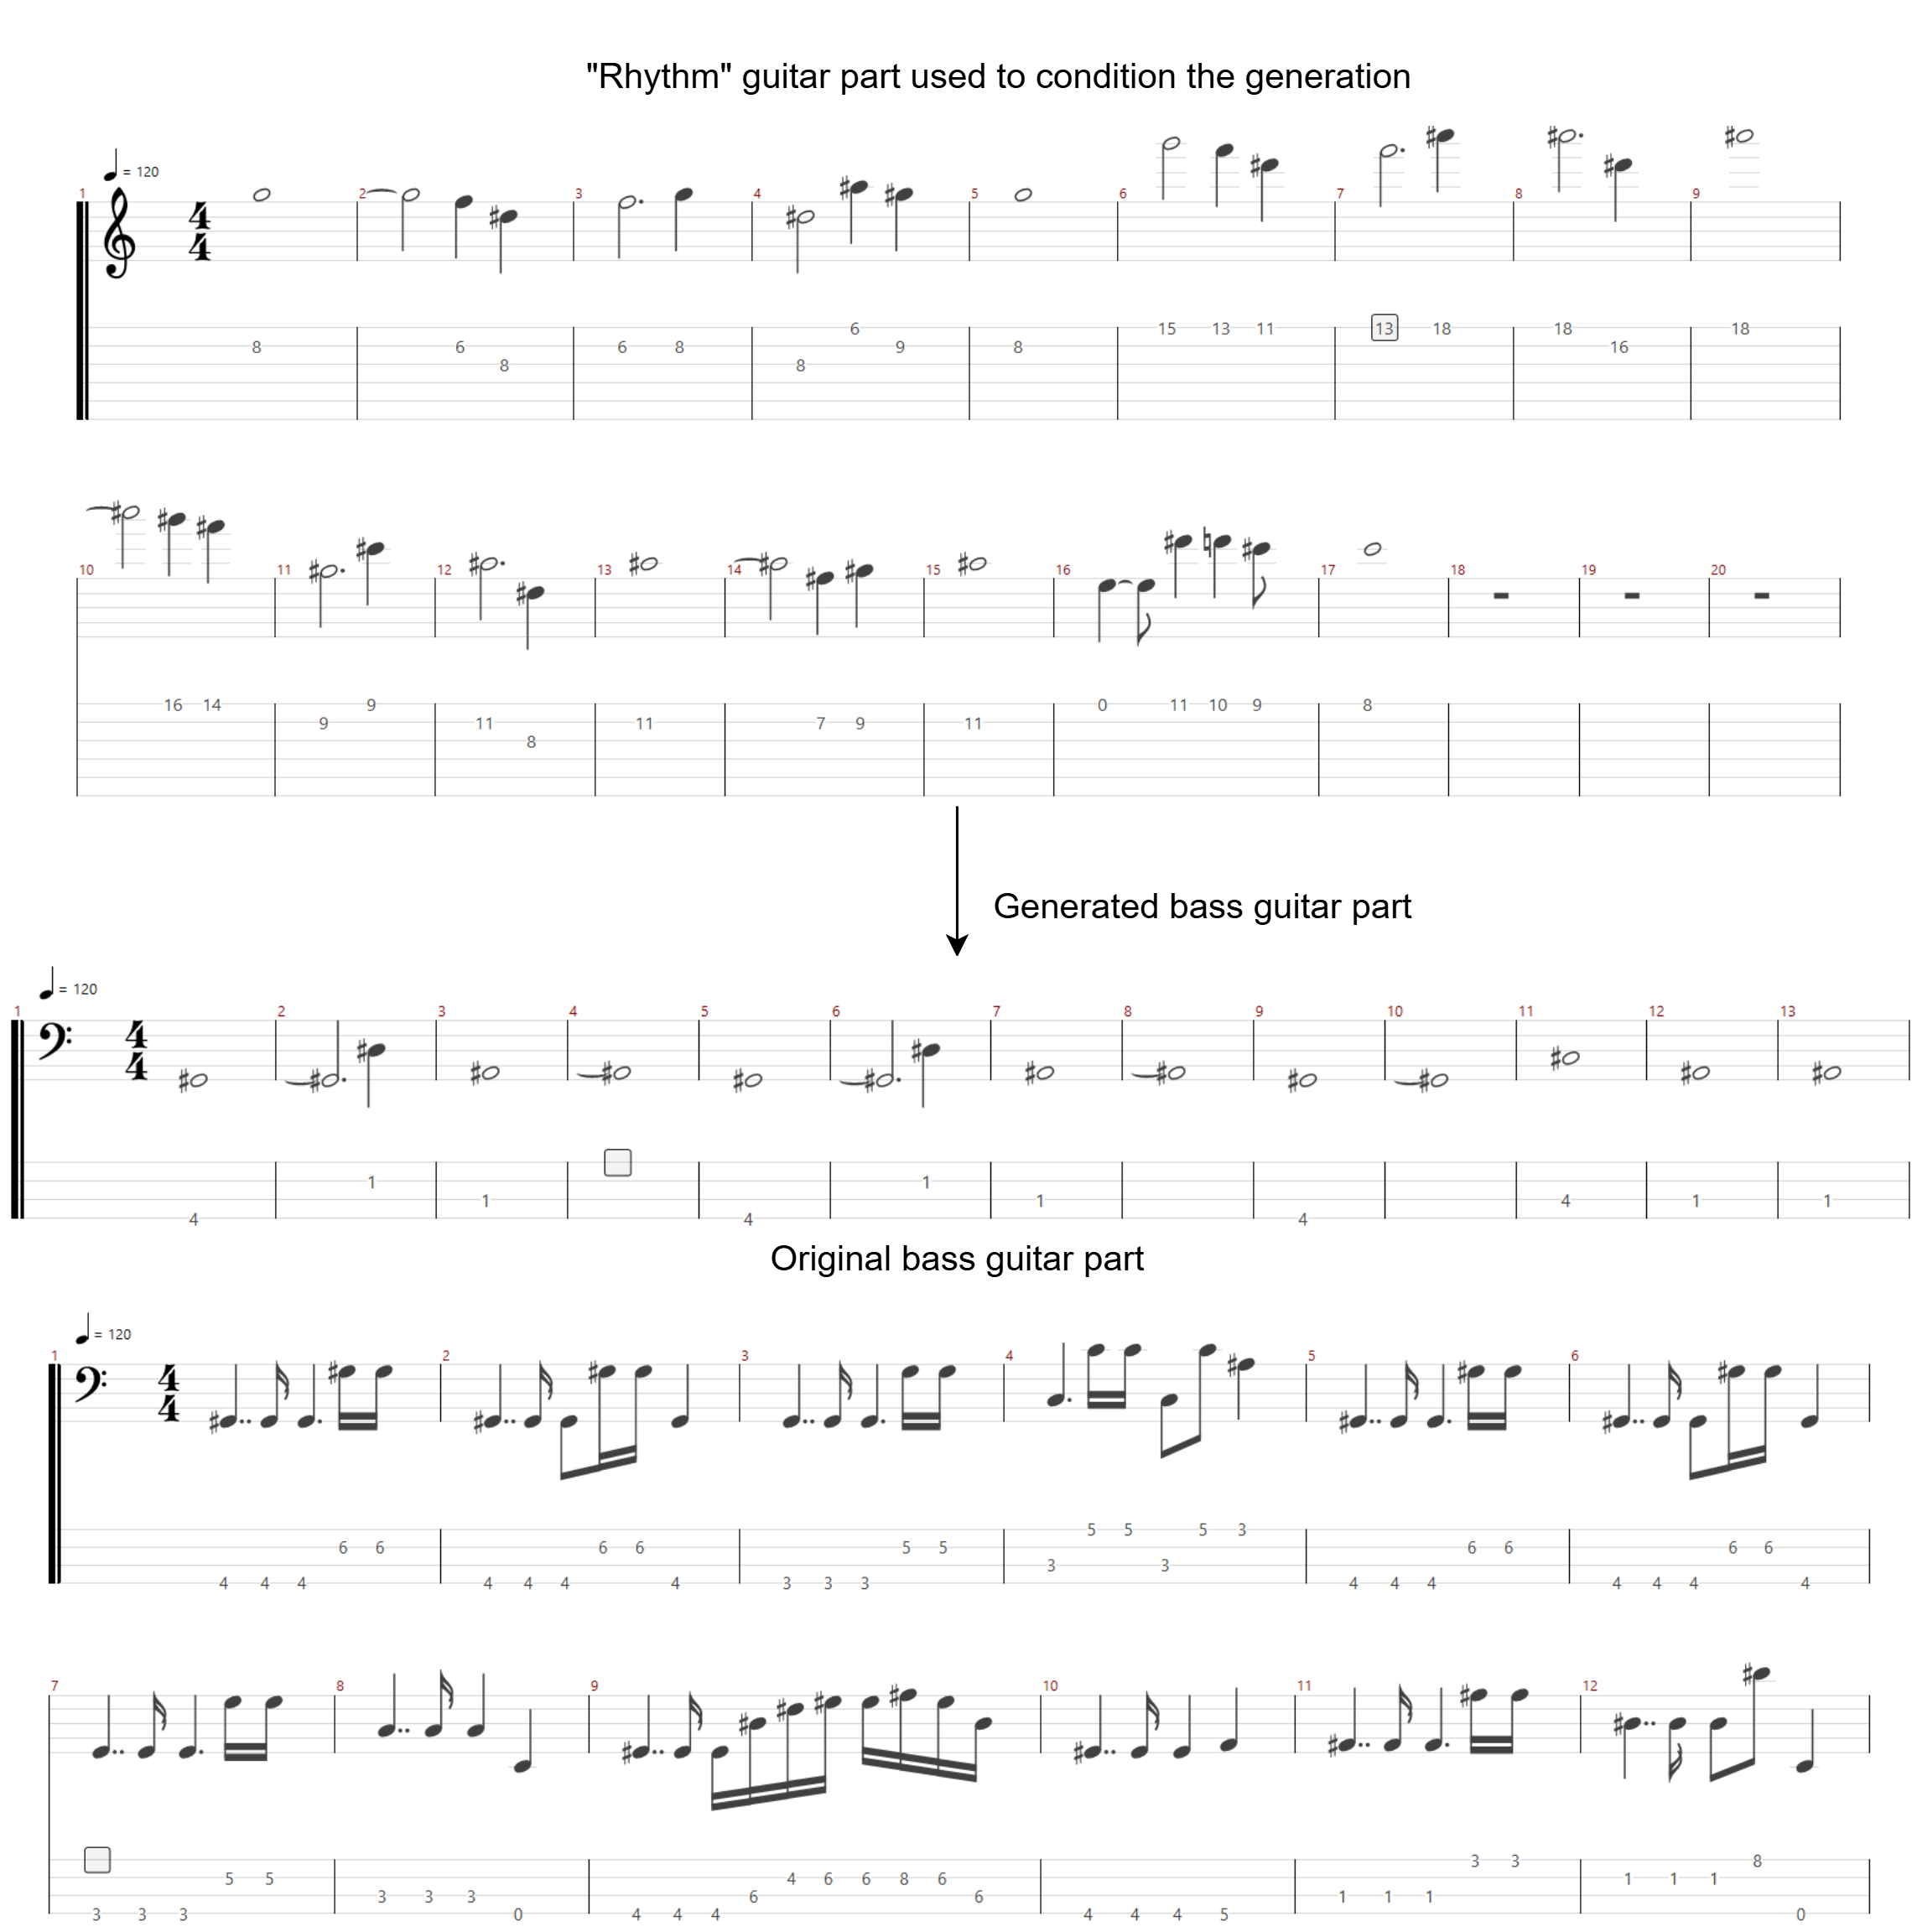
\includegraphics[width=\linewidth]{../images-figures/gen_herbie_hancock.png}
    \caption{Example of 9 measures generated by the model based on the rhythmic guitar part of the song "Saturday Night" by Herbie Hancock}
    \label{fig:gen_herbie_hancock}
\end{figure}

Figure \ref{fig:gen_herbie_hancock} shows an excerpt of bass tablatures generated by the model in the jazz funk genre.
Bass guitar in jazz funk music often plays a more melodic role, with complex rhythmic patterns and harmonies.
Moreover, there are no rhythmic guitar parts strictly speaking in jazz funk music, so the model generates using a more melodic guitar part.
As expected, the generated part is way simpler than the original bass part.
It is meant to be an accompaniment to the guitar part, not a melodic part.
Moreover, jazz funk music often uses complex harmonies, so the model has a hard time following the harmonic progression.
This genre can be considered as a limit case for the model. As it was trained on an agglomerate of genres, it is not able to generate coherent jazz funk bass lines.

To summarize, the model has great potential in generating bass tablatures of accompaniment that are harmonically and rhythmically coherent with the rhythmic guitar part.
However, it struggles to adapt to the specificities of each genre and can still make rhythmical mistakes.
We tried to build an adaptable model that could generate bass lines for a wide range of styles,
but it would be interesting to analyze the model's performance on a specific genre if trained on said genre only.

\subsection{Perspectives}

With additional time, several improvements could be made to the model architecture and tuning, data processing, and evaluation.
One potential enhancement is simplifying the model by removing one of the dense layers in the embedding process, which could reduce complexity without significantly impacting performance.
Additionally, experimenting with compound word tokenization as an alternative to the current DADAGP method might yield more meaningful representations. 

Beyond architectural changes, a user study could be conducted to assess the quality of the generated bass lines, providing valuable insights into the model's musical coherence.
Finally, evaluating the model's environmental impact using Green AI metrics, specifically by measuring the number of floating point operations (FLOPs), would contribute to a better understanding of its computational efficiency.

